\section{HÌNH NÓN} % Tên bài
\subsection{Kiến thức trọng tâm}
\subsubsection{Định nghĩa}
\begin{boxdl}
	\immini{Khi quay tam giác vuông $SOB$ một vòng quanh cạnh góc vuông $SO$ cố định ta được một hình nón (Hình bên).
		\begin{itemize}
			\item $S$ gọi là đỉnh của hình nón.
			\item Cạnh $OB$ quét thành hình tròn gọi là đáy của hình nón.\\
			Bán kính của đáy gọi là bán kính đáy của hình nón.
			\item Cạnh $SB$ quét thành mặt xung quanh của hình nón.\\
			Mỗi vị trí của $SB$ là một đường sinh.
			\item Độ dài $SO$ là chiều cao của hình nón.
	\end{itemize}}
	{\begin{tikzpicture}[line
			join=round,line
			cap=round,font=\scriptsize,>=stealth]
			\def\a{2.4}
			\def\b{1}
			\def\cao{3.7}
			\pgfmathsetmacro\g{asin(\b/\cao)}
			\pgfmathsetmacro\xo{\a *cos(\g)}
			\pgfmathsetmacro\yo{\b *sin(\g)}
			\draw[dashed]
			(\xo,\yo) arc (\g:180-\g:{\a} and
			{\b});
			\path (180:\a)coordinate (A)
			(0:\a) coordinate (B)
			(90:\cao) coordinate (S)
			(0:0)coordinate (O)
			(\xo,\yo)coordinate (M);
			\draw (90:\cao)--(-\xo,\yo) arc
			(180-\g:360+\g:{\a} and
			{\b})--cycle;
			\draw[dashed] (S)--(O)--(B);
			\pic[draw,angle radius=8pt]{right angle=B--O--S};
			\draw[<->,left=0.1] ($ (S)+(-0.1,0) $)--($ (O)+(-0.1,0) $) node[midway,above,rotate=90]{chiều cao};
			\path (S)--(O)node[midway,right]{$h$};
			\path (S)--(B)node[pos=0.6,right]{$l$};
			\path (O)--(B) node[pos=0.5,above]{$r$};
			\draw[<-] ($(S)!0.5!(B)$)--++(2,0)node[midway,above,inner sep=0pt]{đường sinh};
			\draw[<-] (S)--++(145:1)node[above]{đỉnh};
			\draw[<-] ($(O)!0.5!(B)$)--++(2,-1)node[below,inner sep=0pt]{bán kính đáy};
			\foreach\x/\y in {S/90,O/-90,B/0}
			{\fill (\x) circle (1pt)node[shift={(\y:0.3)}]{$\x$};}
			%\path (current bounding box.south)node[below]{Hình 1};
	\end{tikzpicture}}
\end{boxdl}

\subsubsection{Diện tích xung quanh, diện tích toàn phần của hình nón}
	\begin{boxdl}
		Diện tích xung quanh $S_\text{xq}$ của hình nón có bán kính đáy $r$, độ dài đường sinh $l$ là
		$$ S_\text{xq}=\pi rl.$$
		Diện tích toàn phần $S_\text{tp}$ của hình nón có bán kính đáy $r$, độ dài đường sinh $l$ là
		$$S_\text{tp}=\pi rl+\pi r^2.$$
	\end{boxdl}
\subsubsection{Thể tích của hình nón}
	\begin{boxdl}
		Thể tích $V$ của hình nón có bán kính đáy $r$ và chiều cao $h$ là
		$$ V = \dfrac{1}{3}Sh = \dfrac{1}{3}\pi r^2h$$
		với $S$ là diện tích đáy của hình nón.
	\end{boxdl}
	
\subsection{Bài tập}

\begin{vd}%[Dự án EX-9-Đề Cương Toán 9]%[Phạm Hoài]%[9H4H2-1]
	Hãy cho biết bán kính đáy, chiều cao, độ dài đường sinh của mỗi hình nón sau (\textit{kết quả làm tròn đến hàng phần mười của centimét}).
	\begin{center}
		\begin{tabular}{c c c}
			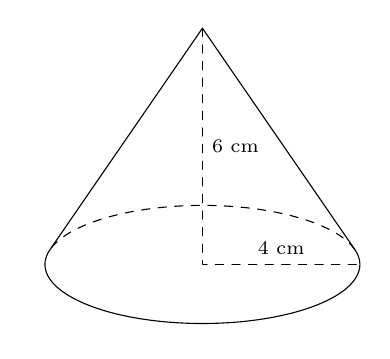
\begin{tikzpicture}[line
				join=round,line
				cap=round,font=\scriptsize,>=stealth]
				\def\a{2}
				\def\b{0.75}
				\def\cao{3}
				\pgfmathsetmacro\g{asin(\b/\cao)}
				\pgfmathsetmacro\xo{\a *cos(\g)}
				\pgfmathsetmacro\yo{\b *sin(\g)}
				\draw[dashed]
				(\xo,\yo) arc (\g:180-\g:{\a} and
				{\b});
				\path (180:\a)coordinate (A)
				(0:\a) coordinate (B)
				(90:\cao) coordinate (S)
				(0:0)coordinate (O)
				(\xo,\yo)coordinate (M);
				\draw (90:\cao)--(-\xo,\yo) arc
				(180-\g:360+\g:{\a} and
				{\b})--cycle;
				\draw[dashed] (S)--(O)--(B);
				\path (S)--(O)node[midway,right]{$6$ cm};
				\path (S)--(B)node[midway,right]{$ $};
				\path (O)--(B)node[midway,above]{$4$ cm};
			\end{tikzpicture}&
			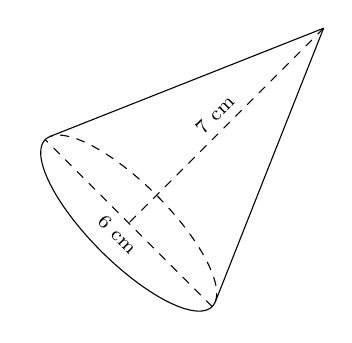
\begin{tikzpicture}[line
				join=round,line
				cap=round,font=\scriptsize,>=stealth,rotate=-45,transform shape]
				\def\a{1.5}
				\def\b{0.5}
				\def\cao{3.5}
				\pgfmathsetmacro\g{asin(\b/\cao)}
				\pgfmathsetmacro\xo{\a *cos(\g)}
				\pgfmathsetmacro\yo{\b *sin(\g)}
				\draw[dashed]
				(\xo,\yo) arc (\g:180-\g:{\a} and
				{\b});
				\path (180:\a)coordinate (A)
				(0:\a) coordinate (B)
				(90:\cao) coordinate (S)
				(0:0)coordinate (O)
				(\xo,\yo)coordinate (M);
				\draw (90:\cao)--(-\xo,\yo) arc
				(180-\g:360+\g:{\a} and
				{\b})--cycle;
				\draw[dashed] (S)--(O) (B)--(A);
				\path (O)--(S)node[midway,sloped,above]{$7$ cm};
				\path (S)--(B)node[midway,right]{$ $};
				\path (A)--(B)node[midway,below]{$6$ cm};
			\end{tikzpicture}&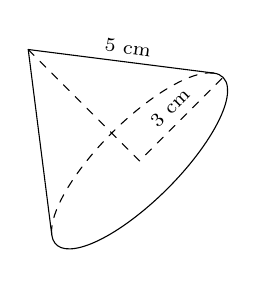
\begin{tikzpicture}[line
				join=round,line
				cap=round,font=\scriptsize,>=stealth,rotate=45,transform shape]
				\def\a{1.5}
				\def\b{0.5}
				\def\cao{2}
				\pgfmathsetmacro\g{asin(\b/\cao)}
				\pgfmathsetmacro\xo{\a *cos(\g)}
				\pgfmathsetmacro\yo{\b *sin(\g)}
				\draw[dashed]
				(\xo,\yo) arc (\g:180-\g:{\a} and
				{\b});
				\path (180:\a)coordinate (A)
				(0:\a) coordinate (B)
				(90:\cao) coordinate (S)
				(0:0)coordinate (O)
				(\xo,\yo)coordinate (M);
				\draw (90:\cao)--(-\xo,\yo) arc
				(180-\g:360+\g:{\a} and
				{\b})--cycle;
				\draw[dashed] (S)--(O)--(B);
				\path (S)--(B)node[midway,sloped,above]{$5$ cm};
				\path (O)--(B)node[midway,above]{$3$ cm};
			\end{tikzpicture}\\
			a)&b)&c)
		\end{tabular}
	\end{center}
	\loigiai{
		Hình a)
		\begin{itemize}
			\item Độ dài đường sinh của hình nón là $l=\sqrt{4^2+6^2} = 2\sqrt{13} \approx 7{,}2$ (cm).
			\item Bán kính đáy, chiều cao, độ dài đường sinh của hình nón lần lượt là $4$ (cm); $6$ (cm); $7{,}2$ (cm).
		\end{itemize}
		Hình b)
		\begin{itemize}
			\item Bán kính đáy của nón là $6\colon 2=3$ cm.\\ 
			Độ dài đường sinh của hình nón là $l=\sqrt{r^2+h^2}=\sqrt{3^2+7^2} = \sqrt{58} \approx 7{,}6$ (cm).
			\item Bán kính đáy, chiều cao, độ dài đường sinh của hình nón lần lượt là $3$ (cm); $7$ (cm); $7{,}6$ (cm).
		\end{itemize}
		Hình c)
		\begin{itemize}
			\item Chiều cao của hình nón là $h =\sqrt{l^2-r^2}=\sqrt{5^2-3^2}=4$ (cm).
			\item Bán kính đáy, chiều cao, độ dài đường sinh của hình nón lần lượt là $3$ (cm); $4$ (cm); $5$ (cm).
		\end{itemize}
	}
\end{vd}

\begin{vd}%[Dự án EX-9-Đề Cương Toán 9]%[Phạm Hoài]%[9H4H2-1]
	Cắt mặt xung quanh của hình nón có chiều cao $9$ cm và bán kính đáy $12$ cm theo một đường sinh của nó rồi trải phẳng ra, ta được một hình quạt tròn. Tính bán kính, độ dài cung của hình quạt tròn đó.
	\loigiai{
		Bán kính $R$ của hình quạt tròn bằng độ dài đường sinh $l$ của hình nón do đó
		\[R =l=\sqrt{h^2+r^2}=\sqrt{9^2+12^2}=15~(\mathrm{cm}).\]
		Độ dài cung $C$ của hình quạt tròn bằng chu vi đáy hình nón do đó
		\[C = 2\pi R = 2\pi\cdot12=24 \pi~(\mathrm{cm}).\]
	}
\end{vd}

\begin{vd}%[Dự án EX-9-Đề Cương Toán 9]%[Phạm Hoài]%[9H4H2-3]
	Cho tam giác $OAB$ vuông tại $O$ có $OB = 20$ cm, $OA = 21$ cm. Tính diện tích xung quanh và thể tích của hình tạo thành khi quay tam giác $OAB$ một vòng quanh cạnh $OB$.
	\loigiai{
		\immini{
			Hình tạo thành khi quay tam giác $OAB$ một vòng quanh cạnh $OB$ là hình nón có bán kính đáy $r =21$ (cm) và chiều cao $h =20$ (cm), suy ra đường sinh $l=\sqrt{20^2+21^2}=29$ (cm).\\
			Diện tích xung quanh của hình nón là
			$$S =\pi rl =\pi \cdot21 \cdot29=609\pi \,  \text{ (cm$^2$).}$$
			Thể tích của hình nón là
			$$V =\dfrac{1}{3} \pi r ^2 h=\dfrac{1}{3}\pi\cdot 21^2\cdot 20 = 2\,940 \pi\, \text{ (cm$^2$).}$$
		}{
			\begin{tikzpicture}[line
				join=round,line
				cap=round,font=\footnotesize,>=stealth]
				\def\a{2.9}
				\def\b{0.75}
				\def\cao{2.8}
				\pgfmathsetmacro\g{asin(\b/\cao)}
				\pgfmathsetmacro\xo{\a *cos(\g)}
				\pgfmathsetmacro\yo{\b *sin(\g)}
				\draw[dashed]
				(\xo,\yo) arc (\g:180-\g:{\a} and
				{\b});
				\path (180:\a)coordinate (A)
				(90:\cao) coordinate (B)
				(0:0)coordinate (O);
				\draw (90:\cao)--(-\xo,\yo) arc
				(180-\g:360+\g:{\a} and
				{\b})--cycle;
				\draw[dashed] (A)--(O)--(B);
				\path (B)--(O)node[midway,right]{$20~\mathrm{cm}$};
				\path (O)--(A)node[midway,above]{$21~\mathrm{cm}$};
				\foreach\x/\y in {B/90,O/-90,A/180}
				{\fill (\x) circle (1pt)node[shift={(\y:0.3)}]{$\x$};}
				\pic[draw,angle radius=2mm]{right angle=B--O--A};
			\end{tikzpicture}
		}
	}
\end{vd}

\begin{vd}%[Dự án EX-9-Đề Cương Toán 9]%[Phạm Hoài]%[9H4H4-1]
	\immini{Người ta dùng tôn để uốn thành một thùng đựng nước hình trụ có nắp là hình nón với các kích thước như hình bên.
		\begin{enumerate}
			\item Tính diện tích tôn cần dùng để làm thùng nước (không tính phần mép dán và hao hụt).
			\item Tính thể tích của thùng (bỏ qua bề dày của tôn).
			(\textit{Làm tròn kết quả đến hàng đơn vị của mét vuông, mét khối}).
	\end{enumerate}}
	{\begin{tikzpicture}[line
			join=round,line
			cap=round,font=\footnotesize,>=stealth]
			\def\a{0.6}
			\def\b{0.2}
			\def\cao{1.3}
			\pgfmathsetmacro\g{asin(\b/\cao)}
			\pgfmathsetmacro\xo{\a *cos(\g)}
			\pgfmathsetmacro\yo{\b *sin(\g)}
			\draw[dashed]
			(\xo,\yo) arc (\g:180-\g:{\a} and
			{\b})
			(\xo,\yo)++(0,-3.5) arc (\g:180-\g:{\a} and
			{\b})
			;
			\path (180:\a)coordinate (A)
			(0:\a) coordinate (B)
			(90:\cao) coordinate (S)
			(0:0)coordinate (O)
			(A)++(0,-3.5) coordinate (C)
			(B)++(0,-3.5) coordinate (D);
			;
			\draw (90:\cao)--(-\xo,\yo) arc
			(180-\g:360+\g:{\a} and
			{\b})--cycle (A)--(C) (B)--(D)
			(-\xo,\yo)++(0,-3.5) arc
			(180-\g:360+\g:{\a} and
			{\b})
			;
			\path (A)--(S)node[midway,above,rotate=64]{$15$ m};
			\draw[<->] ($ (B)+(0.5,0) $)--($ (D)+(0.5,0) $)node[midway,right]{$50$ m};
			\draw[<->] ($ (C)+(0,-0.5) $)--($ (D)+(0,-0.5) $)node[midway,below]{$12$ m};
	\end{tikzpicture}}
	\loigiai{
		\begin{enumerate}
			\item Bán kính đáy thùng nước là $r=12\colon 2=6$ m.\\
			Diện tích xung quanh của phần hình trụ là
			$$ S_1 = 2\pi r h=2\pi\cdot 6\cdot 50 = 600 \pi\, \text{ (m$^2$).}$$
			Diện tích mặt đáy của thùng là $S_2=\pi r^2=\pi \cdot 6^2=36 \pi$ (m$^2$).\\
			Diện tích xung quanh của nắp hình nón là
			$$ S_3 =\pi rl= \pi\cdot 6\cdot15 = 90\pi \,\text{ (m$^2$).} $$
			Diện tích tôn cần dùng là
			$$ S_1 + S_2 + S_3 = 600\pi + 36\pi + 90\pi = 726\pi \approx 2\,281 \, \text{ (m$^2$).}$$
			\item Thể tích của phần hình trụ là $V_1=\pi r^2 h=\pi\cdot 6^2 \cdot 50 = 1\,800\pi$ (m$^3$).\\
			Chiều cao của nắp hình nón là $h =\sqrt{l^2-r^2} =\sqrt{15^2-6^2} = 3\sqrt{21}$ (m).\\
			Thể tích của phần hình nón là
			$$V_2 = \dfrac{1}{3}\pi r^2 h=\dfrac{1}{3}\cdot\pi\cdot 6^2\cdot 3\sqrt{21} = 36\pi\sqrt{21} \text{ (m$^3$).} $$
			Thể tích của chiếc thùng là $V_1+V_2 = 1\,800\pi + 36\pi\sqrt{21} \approx 6\,173$ (m$^3$).
		\end{enumerate}
	}
\end{vd}

\begin{bt}%[Dự án EX-9-Đề Cương Toán 9]%[Phạm Hoài]%[9H4N2-1]
	Trong các hình sau đây, hình nào là hình nón?
	\begin{center}
		\begin{tikzpicture}[scale=.5, font=\footnotesize, line join=round, line cap=round, >=stealth]
			\def\x{2.5} % Bán kính trụ lớn
			\pgfmathsetmacro{\y}{\x/4} % Bán kính trục bé
			\def\h{5} % Chiều cao
			\coordinate (A) at (\x,0);
			\coordinate (O) at (0,0);
			\coordinate (A') at ($(A)+(90:\h)$);
			\coordinate (O') at ($(O)+(90:\h)$);
			\draw (A) arc (0:-180:{\x} and {\y})--($(A')!2!(O')$) arc (180:0:{\x} and {\y}) arc (0:-180:{\x} and {\y}) (A)--(A')--(O');
			\draw[dashed] (O')--(O)--(A) arc (0:180:{\x} and {\y});
			\draw($(O)+(-90:1)$)node[below]{$a)$};
		\end{tikzpicture}\hspace{1cm}
		\begin{tikzpicture}[scale=.5, font=\footnotesize, line join=round, line cap=round, >=stealth]
			\def\x{3} % Bán kính trụ lớn
			\pgfmathsetmacro{\y}{\x/4} % Bán kính trục bé
			\def\h{5} % Chiều cao
			\coordinate (O) at (0,0);
			\coordinate (A) at (\x,0);
			\coordinate (S) at (0,\h);
			\draw (A) arc (0:-180:{\x} and {\y})--(S)--cycle;
			\draw[dashed] (S)--(O)--(A) arc (0:180:{\x} and {\y});
			\draw($(O)+(-90:1)$)node[below]{$b)$};
		\end{tikzpicture}\hspace{1cm}
		\begin{tikzpicture}[scale=.5, font=\footnotesize, line join=round, line cap=round, >=stealth]
			\def\ac{4} % cạnh AC
			\def\ab{2} % cạnh AB
			\def\as{4} % cạnh AS
			\def\gocA{50} % góc A của đáy
			\coordinate (A) at (0,0);
			\coordinate (C) at (\ac,0);
			\coordinate (B) at (-\gocA:\ab);
			\coordinate (S) at (70:\as);
			\draw (A)--(B)--(C)--(S)--cycle (S)--(B);
			\draw[dashed] (A)--(C);
			\draw($(B)+(-90:1)$)node[below]{$c)$};
		\end{tikzpicture}\hspace{1cm}
		\begin{tikzpicture}[scale=.5, font=\footnotesize, line join=round, line cap=round, >=stealth]
			\def\x{3} % Bán kính trụ lớn
			\pgfmathsetmacro{\y}{\x/4} % Bán kính trục bé
			\def\h{5} % Chiều cao
			\coordinate (O) at (0,\h);
			\coordinate (A) at (\x,\h);
			\coordinate (S) at (0,0);
			\draw[dashed] (A) arc (0:-180:{\x} and {\y})--(S)--cycle;
			\draw (A) arc (0:180:{\x} and {\y})--(S)--cycle;
			\draw($(S)+(-90:1)$)node[below]{$d)$};
		\end{tikzpicture}\\Hình 11
	\end{center}
	\loigiai{Hình b) và hình d) là hình nón.}
\end{bt}

\begin{bt}%[Dự án EX-9-Đề Cương Toán 9]%[Phạm Hoài]%[ID]%[Dự án EX-9-Đề Cương Toán 9]%[Phạm Hoài]%[9H4H2-1]
	Hãy cho biết bán kính đáy, chiều cao, độ dài đường sinh của mỗi hình nón sau
	\begin{center}
		\begin{tabular}{c c c}
			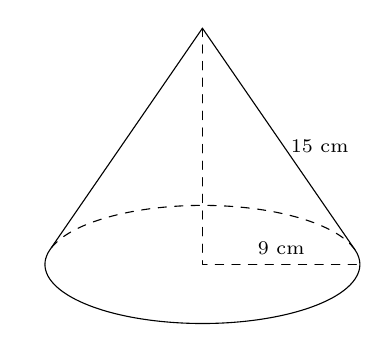
\begin{tikzpicture}[line
				join=round,line
				cap=round,font=\scriptsize,>=stealth]
				\def\a{2}
				\def\b{0.75}
				\def\cao{3}
				\pgfmathsetmacro\g{asin(\b/\cao)}
				\pgfmathsetmacro\xo{\a *cos(\g)}
				\pgfmathsetmacro\yo{\b *sin(\g)}
				\draw[dashed]
				(\xo,\yo) arc (\g:180-\g:{\a} and
				{\b});
				\path (180:\a)coordinate (A)
				(0:\a) coordinate (B)
				(90:\cao) coordinate (S)
				(0:0)coordinate (O)
				(\xo,\yo)coordinate (M);
				\draw (90:\cao)--(-\xo,\yo) arc
				(180-\g:360+\g:{\a} and
				{\b})--cycle;
				\draw[dashed] (S)--(O)--(B);
				\path (S)--(B)node[midway,right]{$15~\mathrm{cm}$};
				\path (O)--(B)node[midway,above]{$9~\mathrm{cm}$};
			\end{tikzpicture}&
			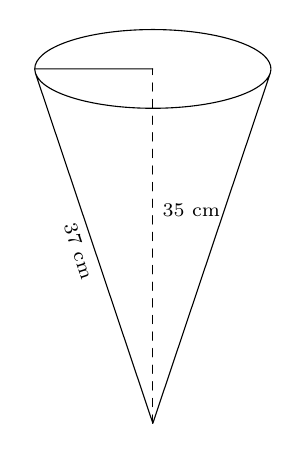
\begin{tikzpicture}[line
				join=round,line
				cap=round,font=\scriptsize,>=stealth]
				\def\a{1.5}
				\def\b{0.5}
				\def\cao{4.5}
				\pgfmathsetmacro\g{asin(\b/\cao)}
				\pgfmathsetmacro\xo{\a *cos(\g)}
				\pgfmathsetmacro\yo{\b *sin(\g)}
				\draw
				(-\xo,-\yo) arc (180+\g:-\g:{\a} and
				{\b});
				\path (180:\a)coordinate (A)
				(0:\a) coordinate (B)
				(-90:\cao) coordinate (S)
				(0:0)coordinate (O)
				(\xo,\yo)coordinate (M);
				\draw (S)--(-\xo,-\yo) arc
				(180+\g:360-\g:{\a} and
				{\b})--cycle
				(A)--(O);
				\draw[dashed] (S)--(O);
				\path (A)--(S)node[midway,sloped,below]{$37~\mathrm{cm}$};
				\path (O)--(S)node[pos=0.4,right]{$35~\mathrm{cm}$};
			\end{tikzpicture}
			&
			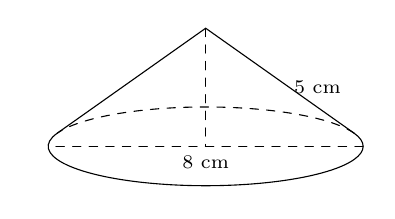
\begin{tikzpicture}[line
				join=round,line
				cap=round,font=\scriptsize,>=stealth]
				\def\a{2}
				\def\b{0.5}
				\def\cao{1.5}
				\pgfmathsetmacro\g{asin(\b/\cao)}
				\pgfmathsetmacro\xo{\a *cos(\g)}
				\pgfmathsetmacro\yo{\b *sin(\g)}
				\draw[dashed]
				(\xo,\yo) arc (\g:180-\g:{\a} and
				{\b});
				\path (180:\a)coordinate (A)
				(0:\a) coordinate (B)
				(90:\cao) coordinate (S)
				(0:0)coordinate (O)
				(\xo,\yo)coordinate (M);
				\draw (90:\cao)--(-\xo,\yo) arc
				(180-\g:360+\g:{\a} and
				{\b})--cycle;
				\draw[dashed] (S)--(O) (B)--(A);
				\path (S)--(B)node[midway,right]{$5$ cm};
				\path (A)--(B)node[midway,below]{$8$ cm};
			\end{tikzpicture}\\
			a)&b)&c)
		\end{tabular}
	\end{center}
	\loigiai{
		Hình a)
		\begin{itemize}
			\item Chiều cao của hình nón là $h=\sqrt{l^2-r^2} =\sqrt{15^2-9^2}=12$ cm.
			\item Bán kính đáy, chiều cao, độ dài đường sinh của hình nón lần lượt là $9$ cm, $12$ cm, $15$ cm.
		\end{itemize}
		Hình b)
		\begin{itemize}
			\item Bán kính đáy của hình nón là $r =\sqrt{l^2-h^2}=\sqrt{37^2-35^2}=12$ cm.
			\item Bán kính đáy, chiều cao, độ dài đường sinh của hình nón lần lượt là $12$ cm, $35$ cm, $37$ cm.
		\end{itemize}
		Hình c)
		\begin{itemize}
			\item 
			Bán kính đáy của nón  $r=8:2=4$ cm.\\
			Chiều cao của hình nón là $h=\sqrt{l^2-r^2} =\sqrt{5^2-4^2}=3$ cm.
			\item Bán kính đáy, chiều cao, độ dài đường sinh của hình nón lần lượt là $4$ cm, $3$ cm, $5$ cm.
		\end{itemize}
	}
\end{bt}

\begin{bt}%[Dự án EX-9-Đề Cương Toán 9]%[Phạm Hoài]%[9H4H2-3]
	Thay dấu \lq\lq?\rq\rq\, bằng giá trị thích hợp và hoàn thành bảng sau vào vở\\
	\renewcommand{\arraystretch}{3.2}
	\begin{tabular}{|>{\centering\arraybackslash}m{4cm} 
			| >{\centering\arraybackslash}m{1.5cm} 
			| >{\centering\arraybackslash}m{1.5cm} 
			| >{\centering\arraybackslash}m{1.5cm} 
			| >{\centering\arraybackslash}m{3cm} 				
			| >{\centering\arraybackslash}m{1.5cm}|
		}
		\hline
		Hình & Bán kính đáy (cm) & Chiều cao (cm) & Độ dài đường sinh (cm) & Diện tích xung quanh (cm$^{2}$)& Thể tích (cm$^{3}$) \\
		\hline
		\multirow{2}{*}{
			\begin{tikzpicture}[scale=0.8, font=\footnotesize,>=stealth]
				%Gán số liệu.
				\def\a{2};\def\b{0.6};\def\h{3};
				%Gán tọa độ.
				\coordinate (O) at (0,0);
				\coordinate (S) at ($(O)+(0,\h)$);
				\coordinate (M) at ($(O)-(\a,0)$);
				\coordinate (N) at ($(O)+(\a,0)$);
				%Vẽ khối nón.
				\draw (M) arc (-180:0:\a cm and \b cm) (M)--(S)--(N);
				\draw[dashed] (S)--(O) (M)--(N) (M) arc (180:0:\a cm and \b cm);
				%kí hiệu
				\path(S)--(N)node[midway, right]{$l$};
				\path(S)--(O)node[midway,right]{$h$};
				\path(N)--(O)node[midway, sloped, above]{$R$};
				\draw pic[draw, angle radius=2mm, angle eccentricity=1.5]{right angle = S--O--N};
				%Gọi tên điểm.
				%\foreach \x/\y in {S/90,O/140,M/180,N/0}{\fill (\x) circle (1pt) ($(\x)+(\y:0.3cm)$) node{$\x$};}
			\end{tikzpicture}
		} & $6$ & $8$ & ? & ?&? \\
		\cline{2-6}
		& ? &?& $13$ &$65\pi$&? \\
		\hline
	\end{tabular}
	\loigiai{
		\renewcommand{\arraystretch}{3.2}
		\begin{tabular}{|>{\centering\arraybackslash}m{4cm} 
				| >{\centering\arraybackslash}m{1.5cm} 
				| >{\centering\arraybackslash}m{1.5cm} 
				| >{\centering\arraybackslash}m{1.5cm} 
				| >{\centering\arraybackslash}m{3cm} 				
				| >{\centering\arraybackslash}m{1.5cm}|
			}
			\hline
			Hình & Bán kính đáy (cm) & Chiều cao (cm) & Độ dài đường sinh (cm) & Diện tích xung quanh (cm$^{2}$)& Thể tích (cm$^{3}$) \\
			\hline
			\multirow{2}{*}{
				\begin{tikzpicture}[scale=0.8, font=\footnotesize,>=stealth]
					%Gán số liệu.
					\def\a{2};\def\b{0.6};\def\h{3};
					%Gán tọa độ.
					\coordinate (O) at (0,0);
					\coordinate (S) at ($(O)+(0,\h)$);
					\coordinate (M) at ($(O)-(\a,0)$);
					\coordinate (N) at ($(O)+(\a,0)$);
					%Vẽ khối nón.
					\draw (M) arc (-180:0:\a cm and \b cm) (M)--(S)--(N);
					\draw[dashed] (S)--(O) (M)--(N) (M) arc (180:0:\a cm and \b cm);
					%kí hiệu
					\path(S)--(N)node[midway, right]{$l$};
					\path(S)--(O)node[midway,right]{$h$};
					\path(N)--(O)node[midway, sloped, above]{$R$};
					\draw pic[draw, angle radius=2mm, angle eccentricity=1.5]{right angle = S--O--N};
					%Gọi tên điểm.
					%\foreach \x/\y in {S/90,O/140,M/180,N/0}{\fill (\x) circle (1pt) ($(\x)+(\y:0.3cm)$) node{$\x$};}
				\end{tikzpicture}
			} & $6$ & $8$ & $10$ & $60\pi$&$96\pi$ \\
			\cline{2-6}
			& $5$ &$12$& $13$ &$65\pi$&$100\pi$ \\
			\hline
		\end{tabular}
	}
\end{bt}

\begin{bt}%[Dự án EX-9-Đề Cương Toán 9]%[Phạm Hoài]%[9H4N2-1]
	Tìm các hình ảnh hình nón trong thực tế.
	\loigiai{
		Một số hình ảnh hình nón trong thực tế là nón lá, chiếc kem, đống cát, $\ldots$
	}
\end{bt}

\begin{bt}%[Dự án EX-9-Đề Cương Toán 9]%[Phạm Hoài]%[ID]
	Tạo lập hình nón có bán kính đáy bằng $4$ cm, chiều cao bằng $7$ cm.
	\loigiai{Tạo lập hình nón có chiều cao $7$ cm và bán kính đáy $4$ cm theo hướng dẫn sau
		\begin{itemize}
			\item Cắt tấm bìa hình quạt tròn có bán kính bằng độ dài đường sinh $l=\sqrt{4^2+7^2}\approx8$ (cm), độ dài cung của hình quạt tròn bằng $2\pi\cdot4\approx25$ cm (Hình a).
			\item Cắt tấm bìa hình tròn bán kính $4$ cm.
			\item Ghép và dán hai mép hình quạt tròn lại với nhau sao cho cung của nó tạo thành đường tròn, rồi dán tấm bìa hình tròn ở trên vào làm đáy, ta được hình nón như Hình b.
		\end{itemize}
		\begin{center}
			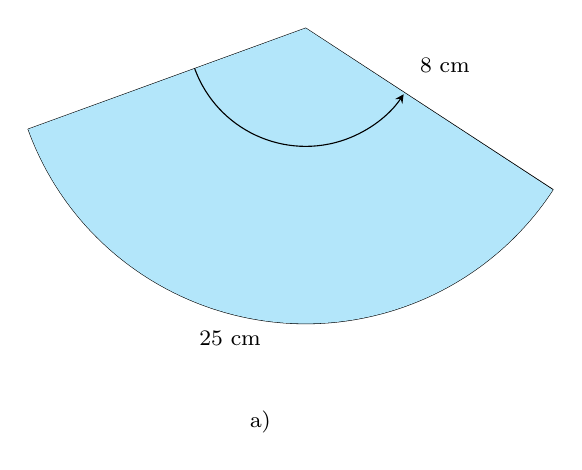
\begin{tikzpicture}[>=stealth,line join=round,line cap=round,font=\footnotesize,scale=.75
				,rotate=200
				]
				%	\draw[thin,gray!50,step=1cm] (-5,-5) grid (5,5);
				
				\coordinate (A) at (0,0);
				\coordinate (B) at (-3,4);
				\coordinate (C) at (5,0);
				\draw (B)--(A)--(C);
				\draw (C) arc (0:126.8:5cm); 
				\fill[cyan!30](A)--(C)arc(0:126.8:5cm)--cycle;
				\draw[->] (2,0) arc (0:126:2cm);
				\draw (-2,1.4) node[]{$8$ cm};
				\draw (3,4.5) node[]{$25$ cm};
				\draw (3,6) node[]{a)};
			\end{tikzpicture}
			\begin{tikzpicture}[scale=.75, font=\footnotesize, line join=round, line cap=round, >=stealth]
				\def\x{3} % Bán kính trụ lớn
				\pgfmathsetmacro{\y}{\x/4} % Bán kính trục bé
				\def\h{5} % Chiều cao
				\coordinate (O) at (0,0);
				\coordinate (A) at (\x,0);
				\coordinate (S) at (0,\h);
				\draw($(S)!.5!(O)+(180:\x)$)node[left]{$\Longrightarrow$};
				\draw (A) arc (0:-180:{\x} and {\y})--(S)--cycle;
				\draw[dashed] (S)--(O)node[midway, right]{$7\mathrm{~cm}$}--(A)node[midway, above]{$4\mathrm{~cm}$} arc (0:180:{\x} and {\y});
				\foreach \diem in {A,S,O}	\fill (\diem)circle(1.5pt);
				\coordinate[label=below:$\text{b)}$] (F) at ($(O)+(-90:1)$);
				\draw pic[draw,blue,angle radius=3mm] {right angle = S--O--A}; 
			\end{tikzpicture}
	\end{center}}
\end{bt}

\begin{bt}%[Dự án EX-9-Đề Cương Toán 9]%[Phạm Hoài]%[9H4H2-1]
	Một hình quạt tròn có bán kính $29$ cm, độ dài cung bằng $42 \pi$ cm. Người ta dùng hình quạt tròn này để tạo lập mặt xung quanh của một hình nón. Tính bán kính đáy và chiều cao của hình nón đó.
	\loigiai{
		Gọi $r$ là bán kính đáy của hình nón, độ dài cung của hình quạt tròn bằng chu vi đáy của hình nón, khi đó t có  $2 \pi r =42 \pi$, suy ra $r =21$ (cm).\\
		Độ dài đường sinh $l$ của hình nón bằng bán kính của hình quạt tròn, suy ra $l=29$ (cm).\\
		Chiều cao của hình nón là $h =\sqrt{l^2-r^2}=\sqrt{29^2-21^2}=20$ (cm).\\
		Vậy bán kính đáy và chiều cao của hình nón lần lượt là $21$ cm và $20$ cm.
	}
\end{bt}

\begin{bt}%[Dự án EX-9-Đề Cương Toán 9]%[Phạm Hoài]%[9H4H2-3]
	Cho tam giác $OAB$ vuông tại $O$ có $AB=37$ cm, $OA=12$ cm. Tính diện tích xung quanh và thể tích của hình tạo thành khi quay tam giác $OAB$ một vòng quanh cạnh $OB$.
	\loigiai{
		\begin{center}
			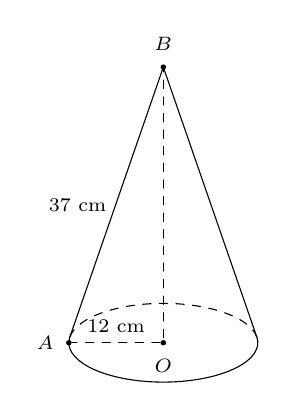
\begin{tikzpicture}[line
				join=round,line
				cap=round,font=\scriptsize,>=stealth]
				\def\a{1.2}
				\def\b{0.5}
				\def\cao{3.5}
				\pgfmathsetmacro\g{asin(\b/\cao)}
				\pgfmathsetmacro\xo{\a *cos(\g)}
				\pgfmathsetmacro\yo{\b *sin(\g)}
				\draw[dashed]
				(\xo,\yo) arc (\g:180-\g:{\a} and
				{\b});
				\path (180:\a)coordinate (A)
				(90:\cao) coordinate (B)
				(0:0)coordinate (O);
				\draw (90:\cao)--(-\xo,\yo) arc
				(180-\g:360+\g:{\a} and
				{\b})--cycle;
				\draw[dashed] (A)--(O)--(B);
				\path (A)--(B)node[midway,left]{$37~\mathrm{cm}$};
				\path (O)--(A)node[midway,above]{$12~\mathrm{cm}$};
				\foreach\x/\y in {B/90,O/-90,A/180}
				{\fill (\x) circle (1pt)node[shift={(\y:0.3)}]{$\x$};}
			\end{tikzpicture}
		\end{center}
		Hình tạo thành là một hình nón có bán kính đáy $r =12$ (cm) và đường sinh $l=37$ (cm), suy ra chiều cao của hình nón là $h=\sqrt{l^2-r^2} =\sqrt{37^2-12^2}=35$ (cm).\\
		Diện tích xung quanh của hình nón là $S =\pi rl=\pi \cdot 12 \cdot 37=444 \pi$ (cm$^2$).\\
		Thể tích của hình nón là $V =\dfrac{1}{3} \pi r ^2 h=\dfrac{1}{3} \cdot \pi \cdot 12^2 \cdot 35=1\,680 \pi$ (cm$^3$).
	}
\end{bt}

\begin{bt}%[Dự án EX-9-Đề Cương Toán 9]%[Phạm Hoài]%[9H4H2-2]
	Hãy cho biết chiều cao, bán kính đáy, độ dài đường sinh và diện tích xung quanh của mỗi hình nón sau
	\begin{center}
		\begin{tikzpicture}[scale=.8, font=\footnotesize, line join=round, line cap=round, >=stealth]
			\def\x{3} % Bán kính trụ lớn
			\pgfmathsetmacro{\y}{\x/4} % Bán kính trục bé
			\def\h{5} % Chiều cao
			\coordinate (O) at (0,0);
			\coordinate (A) at (\x,0);
			\coordinate (S) at (0,\h);
			\draw (A) arc (0:-180:{\x} and {\y})--(S)--cycle;
			\draw[dashed] (S)--(O)node[midway, right]{$6\mathrm{~cm}$}--(A)node[midway, above]{$3\mathrm{~cm}$} arc (0:180:{\x} and {\y});
			\foreach \diem in {A,S,O}	\fill (\diem)circle(1.5pt);
			\draw pic[draw,blue,angle radius=3mm] {right angle = S--O--A}; 
			\coordinate[label=below:$\text{a)}$] (F) at ($(O)+(-90:1)$);
		\end{tikzpicture}\hspace{.75cm}
		\begin{tikzpicture}[scale=.8, font=\footnotesize, line join=round, line cap=round, >=stealth]
			\def\x{3} % Bán kính trụ lớn
			\pgfmathsetmacro{\y}{\x/4} % Bán kính trục bé
			\def\h{5} % Chiều cao
			\coordinate (O) at (0,0);
			\coordinate (A) at (\x,0);
			\coordinate (S) at (0,\h);
			\draw (A) arc (0:-180:{\x} and {\y})--(S)--cyclenode[midway, above right]{$5\mathrm{~cm}$};
			\draw[dashed] (S)--(O)--(A)node[midway, above]{$3\mathrm{~cm}$} arc (0:180:{\x} and {\y});
			\foreach \diem in {A,S,O}	\fill (\diem)circle(1.5pt);
			\draw pic[draw,blue,angle radius=3mm] {right angle = S--O--A}; 
			\coordinate[label=below:$\text{b)}$] (F) at ($(O)+(-90:1)$);
		\end{tikzpicture}\hspace{.75cm}
		\begin{tikzpicture}[scale=.8, font=\footnotesize, line join=round, line cap=round, >=stealth]
			\def\x{3} % Bán kính trụ lớn
			\pgfmathsetmacro{\y}{\x/4} % Bán kính trục bé
			\def\h{5} % Chiều cao
			\coordinate (O) at (0,0);
			\coordinate (A) at (\x,0);
			\coordinate (S) at (0,\h);
			\draw (A) arc (0:-180:{\x} and {\y})--(S)--cyclenode[midway, above right]{$15\mathrm{~cm}$};
			\draw[dashed] (S)--(O)--(A)node[midway, above]{$9\mathrm{~cm}$} arc (0:180:{\x} and {\y});
			\foreach \diem in {A,S,O}	\fill (\diem)circle(1.5pt);
			\draw pic[draw,blue,angle radius=3mm] {right angle = S--O--A}; 
			\coordinate[label=below:$\text{c)}$] (F) at ($(O)+(-90:1)$);
		\end{tikzpicture}
	\end{center}
	\loigiai{
		\begin{enumerate}
			\item Hình nón ở hình a) có bán kính đáy $r=3$ cm, chiều cao $h=6$ cm và độ dài đường sinh bằng $l=\sqrt{r^2+h^2}=\sqrt{3^2+6^2}=3\sqrt{5}$ cm.\\
			Diện tích xung quanh của hình nón là $S_{\text{xq}}=\pi rl=\pi\cdot3\cdot3\sqrt{5}=9\pi\sqrt{5}$ cm$^2$.
			\item Hình nón ở hình b) có bán kính đáy $r=3$ cm, độ dài đường sinh $l=5$ cm và chiều cao bằng $h=\sqrt{l^2-r^2}=\sqrt{5^2-3^2}=4$ cm.\\
			Diện tích xung quanh của hình nón là $S_{\text{xq}}=\pi rl=\pi\cdot3\cdot5=15\pi$ cm$^2$.
			\item Hình nón ở hình c) có bán kính đáy $r=9$ cm, độ dài đường sinh $l=15$ cm và chiều cao bằng $h=\sqrt{l^2-r^2}=\sqrt{15^2-9^2}=12$ cm.\\
			Diện tích xung quanh của hình nón là $S_{\text{xq}}=\pi rl=\pi\cdot9\cdot15=135\pi$ cm$^2$.
		\end{enumerate}
	}
\end{bt}

\begin{bt}%[Dự án EX-9-Đề Cương Toán 9]%[Phạm Hoài]%[9H4H2-3]
	Tính thể tích của hình nón cho biết
	\begin{enumerate}
		\item Bán kính đáy $6$ cm, chiều cao $12$ cm;
		\item Đường kính của mặt đáy là $7$ cm, chiều cao $10$ cm;
		\item Diện tích đáy $152$ cm$^2$, chiều cao $6$ cm;
		\item Chu vi đáy $130$ cm, chiều cao $24$ cm.
	\end{enumerate}	
	\loigiai{
		\begin{enumerate}
			\item Thể tích hình nón là $V=\dfrac{1}{3}\pi r^2h=\dfrac{1}{3}\cdot\pi\cdot6^2\cdot12=144\pi$ (cm$^3$).
			\item Bán kính đáy $r=\dfrac{d}{2}=\dfrac{7}{2}$ cm.\\
			Thể tích hình nón là $V=\dfrac{1}{3}\pi r^2h=\dfrac{1}{3}\cdot\pi\cdot\left(\dfrac{7}{2}\right)^2\cdot10=\dfrac{245\pi}{6}$ (cm$^3$).
			\item Thể tích hình nón là $V=\dfrac{1}{3}Sh=\dfrac{1}{3}\cdot152\cdot6=304$ (cm$^3$).
			\item Chu vi đáy $2\pi r=130 \mathrm{~cm}$ nên $r=\dfrac{65}{\pi}$ (cm).\\
			Thể tích hình nón là $V=\dfrac{1}{3}\pi r^2h=\dfrac{1}{3}\cdot\pi\cdot\left(\dfrac{65}{\pi}\right)^2\cdot24=\dfrac{33\,800}{\pi}$ (cm$^3$).
		\end{enumerate}
	}
\end{bt}

\begin{bt}%[Dự án EX-9-Đề Cương Toán 9]%[Phạm Hoài]%[9H4H2-2]
	Một hình nón có chiều cao là $8$ cm và đường kính đường tròn đáy bằng $12$ cm. Tính diện tích xung quanh của hình nón đó.
	\loigiai{
		Do đường kính đường tròn đáy bằng $12$ cm nên bán kính đường tròn đáy là $r=6$ cm.\\
		Đường sinh của hình nón là
		$l=\sqrt{r^2+h^2}=\sqrt{6^2+8^2}=10$ cm.\\
		Diện tích xung quanh của hình nón là 
		$ \pi\cdot 6\cdot 10 = 60\pi$ cm$^2$. 
	}
\end{bt}

\begin{bt}%[Dự án EX-9-Đề Cương Toán 9]%[Phạm Hoài]%[9H4H2-2]
	Cho hình nón $(N)$ có đường kính đường tròn đáy bằng $4a$, đường sinh bằng $5a$. Tính diện tích xung quanh của hình nón $(N)$.
	\loigiai{
		Do đường kính đường tròn đáy bằng $4a$ cm nên bán kính đường tròn đáy là $r=2a$.\\
		Diện tích xung quanh của hình nón  $(N)$ là 
		$ \pi\cdot 2a\cdot 5a = 10a^2\pi$. 
	}
\end{bt}

\begin{bt}%[Dự án EX-9-Đề Cương Toán 9]%[Phạm Hoài]%[9H4H2-2]
	Một hình nón có đường sinh dài $15$ cm và diện tích xung quanh là $135 \pi$ cm$^2$.
	\begin{enumerate}
		\item Tính diện tích toàn phần của hình nón đó.
		\item Tính chiều cao của hình nón đó.
	\end{enumerate}
	\loigiai{
		\begin{enumerate}
			\item Ta có $S_{\text{xq}}=\pi rl$ suy ra $r = \dfrac{S_{\text{xq}}}{\pi l}=\dfrac{135\pi}{\pi\cdot 15} = 9$ (cm).\\
			Diện tích toàn phần của hình nón đó là
			$S_{\text{tp}}=S_{\text{xq}}+\pi r^2=135\pi + \pi\cdot 9^2 = 216\pi$ (cm$^2$).
			\item Chiều cao của hình nón đó là $h=\sqrt{l^2-r^2}=\sqrt{15^2-9^2}=12$ (cm).
		\end{enumerate}
	}
\end{bt}

\begin{bt}%[Dự án EX-9-Đề Cương Toán 9]%[Phạm Hoài]%[9H4V2-2]
	Một hình nón có diện tích xung quanh và diện tích toàn phần lần lượt bằng $65\pi$ cm$^2$, $115\pi$ cm$^2$. Hỏi chiều cao của hình nón đó bằng bao nhiêu centimét (\textit{làm tròn kết quả đến hàng đơn vị}).
	\loigiai{
		Ta có $S_{\text{tp}}-S_{\text{xq}}=\pi r^2= 115\pi - 65\pi=50\pi$ suy ra $r=\sqrt{50}=5\sqrt{2}$ (cm).\\
		Mà $S_{\text{xq}}=\pi rl = 5\sqrt{2}\pi l=65\pi$ suy ra $=\dfrac{13\sqrt{2}}{2}$ (cm).\\
		Chiều cao của hình nón đó là $h=\sqrt{l^2-r^2}=\sqrt{\left(\dfrac{13\sqrt{2}}{2}\right)^2-\left(5\sqrt{2}\right)^2}=\dfrac{\sqrt{138}}{2}\approx 6$ (cm).
	}
\end{bt}

\begin{bt}%[Dự án EX-9-Đề Cương Toán 9]%[Phạm Hoài]%[9H4V2-2]
	\immini{Khi quay tam giác $OHA$ vuông cân ở $H$ một vòng xung quanh đường thẳng cố định $OH$, ta được một hình nón như ở hình bên. Hỏi diện tích xung quanh của hình nón đó là bao nhiêu centimét vuông (\textit{làm tròn kết quả đến hàng đơn vị})? Biết diện tích tam giác $OHA$ là $4$ cm$^2$.}
	{\begin{tikzpicture}[scale=.75, font=\footnotesize, line join=round, line cap=round, >=stealth]
			\def\x{3} % Bán kính trụ lớn
			\pgfmathsetmacro{\y}{\x/4} % Bán kính trục bé
			\def\h{3} % Chiều cao
			\coordinate[label=below:$H$] (H) at (0,0);
			\coordinate[label=right:$A$] (A) at (\x,0);
			\coordinate[label=above:$O$] (O) at (0,\h);
			%\coordinate[label=left:$B$] (B) at (-\x,0);
			%\coordinate[label=below left:$D$] (D) at ($(O)+(240:{\x} and {\y})$);
			\coordinate[label=below:$ $] (F) at ($(H)+(-90:1)$);	
			\draw (A) arc (0:-180:{\x} and {\y})--(O)--cycle
			(A)
			;
			\draw[dashed] (O)--(H)node[midway, right]{}--(A)node[midway, above]{} arc (0:180:{\x} and {\y});
			\foreach \diem in {A,H,O}	\fill (\diem)circle(1.5pt);
			\draw pic[draw,angle radius=2mm] {right angle = O--H--A}; 
	\end{tikzpicture}}
	\loigiai{
		Vì $\triangle OHA$ cân tại $H$ nên $OH=HA$.\\
		Ta có $S_{OHA}=\dfrac{1}{2}OH\cdot HA=\dfrac{1}{2}HA^2=4$ suy ra $HA=OH=2\sqrt{2}$ (cm).\\
		Đường sinh của hình nón là
		$l=OA=\sqrt{OH^2+HA^2}=4$ (cm).\\
		Diện tích xung quanh của hình nón là
		$S_{\text{xq}}=\pi rl = \pi\cdot 2\sqrt{2}\cdot 4 = 8\sqrt{2}\pi\approx 36$ (cm$^2$).
	}
\end{bt}

\begin{bt}%[Dự án EX-9-Đề Cương Toán 9]%[Phạm Hoài]%[9H4V2-2]
	\immini{
		Cho tam giác vuông $AMC$ vuông tại $M$ có $AC=2MC$ và $AM=3\sqrt{3}$ dm. Khi quay một vòng tam giác $AMC$ xung quanh đường thẳng cố định $AM$, ta có một hình nón như Hình $11$. Tính diện tích toàn phần của hình nón đó (\textit{theo đơn vị decimét vuông và làm tròn kết quả đến hàng phần trăm}).}{
		\begin{tikzpicture}[scale=1, line join = round, line cap = round,font=\footnotesize]
			\pgfmathsetmacro \x{2}  %bán kính trục lớn elip 
			\pgfmathsetmacro \y{0.43}  %bán kính trục bé elip 
			\pgfmathsetmacro \h{2.7}  %chiều cao hình nón 
			\coordinate[label = below:$M$] (O) at (0,0); 
			\coordinate [label = below right:$C$](A) at ($(O)+(\x,0)$); 
			\coordinate (B) at ($(O)-(\x,0)$); 
			\coordinate[label = above:$A$] (S) at ($(O)+(0,\h)$); 
			\draw[dashed] (A) arc (0:180:\x cm and \y cm); 
			\draw (A) arc (0:-180:\x cm and \y cm); 
			\draw(B)--(S)--(A); 
			\draw[dashed](S)--(O)--(A); 
			\foreach \x in {O,A,S,B} \fill (\x) circle (1.0pt);	 
			\node at ($(O)!.5!(S)$) [left] {$h$}; 
			\node at ($(O)!.5!(A)$) [below] {$r$}; 
			\draw  pic [draw, angle radius = 3 mm] {right angle = S--O--A}; 
	\end{tikzpicture}}
	\loigiai{
		Tam giác $AMC$ vuông tại $M$ có $AC=2MC$ nên $\cos \widehat{ACM}=\dfrac{MC}{AC}=\dfrac{1}{2}$. \\
		Do đó, ta có $\widehat{ACM}=60^{\circ}$. \\
		Suy ra $AC=\dfrac{AM}{\sin \widehat{ACM}}=\dfrac{3 \sqrt{3}}{\sin 60^{\circ}}=6$ (dm) và $MC=\dfrac{1}{2} AC=3$ (dm).\\
		Vậy diện tích toàn phần của hình nón đó là $\pi\cdot 3\cdot6 + \pi\cdot 3^2 = 27\pi \approx 84{,}82$ (dm$^2$). 
	}
\end{bt}

\begin{bt}%[Dự án EX-9-Đề Cương Toán 9]%[Phạm Hoài]%[9H4V2-4]
	Bạn Trang làm một chiếc mũ sinh nhật bằng giấy bìa màu, đường kính đáy bằng $16$ cm, độ dài đường sinh bằng $17$ cm. Tính diện tích bìa màu bạn Trang cần dùng để làm chiếc mũ sinh nhật đó (\textit{coi mép dán không đáng kể, làm tròn kết quả đến hàng đơn vị của cm$^2$}).
	\loigiai{
		\immini{
			Bán kính đáy của chiếc mũ hình nón là 
			\[r=16:2=8 \left(\mathrm{cm}\right). \]
			Diện tích giấy bia màu bạn Trang cần dùng là 
			\[S=\pi rl = \pi\cdot 8\cdot 17 = 136\pi\approx 427\left( \mathrm{cm^2}\right).\]\\
		}{
			\begin{tikzpicture}[scale=1, font=\footnotesize,>=stealth]
				%Gán số liệu.
				\def\a{2};\def\b{0.6};\def\h{4};
				%Gán tọa độ.
				\coordinate (O) at (0,0);
				\coordinate (S) at ($(O)+(0,\h)$);
				\coordinate (A) at ($(O)-(\a,0)$);
				\coordinate (B) at ($(O)+(\a,0)$);
				%Vẽ khối nón.
				\draw (A) arc (-180:0:\a cm and \b cm) (A)--(S)--(B);
				\draw[dashed] (S)--(O) (A)--(B) (A) arc (180:0:\a cm and \b cm);
				\path(S)--(B)node[sloped, midway, above]{$17$ cm};
				\path(A)--(B)node[sloped, midway, below]{$16$ cm};
				%Gọi tên điểm.
				%\foreach \x/\y in {S/90,O/140,A/180,B/0}{\fill (\x) circle (1pt) ($(\x)+(\y:0.3cm)$) node{$\x$};}
			\end{tikzpicture}
		}
	}
\end{bt} 

\begin{bt}%[Dự án EX-9-Đề Cương Toán 9]%[Phạm Hoài]%[9H4V2-4]
	\immini{
		Công trình Trung tâm triển lãm văn hoá nghệ thuật và nhà hát Cao Văn Lầu (tỉnh Bạc Liêu) được xây dựng với tổng diện tích $2\,262$ m$^2$ và được chia thành ba khối có dạng hình trụ tròn tương ứng với ba mái dạng hình chiếc nón lá hướng vào nhau. Chiều cao và đường kính đáy của mái dạng hình chiếc nón lớn nhất trong ba mái hình chiếc nón lần lượt là $24{,}25$ m và $45{,}15$ m. Tính thể tích của mái hình chiếc nón lớn nhất đó theo đơn vị mét khối (\textit{làm tròn kết quả đến hàng phần mười}).
	}{
		\includegraphics[scale=0.5]{Images/9C9-B2-CaoVanLau}
	}
	\loigiai{
		Thể tích của mái hình chiếc nón lớn nhất đó là
		$$
		V=\dfrac{1}{3} \cdot \pi \cdot\left(\dfrac{45{,}15}{2}\right)^2 \cdot 24{,}25 \approx 12\,941{,}8 \text{ (m$^3$).}
		$$
	}
\end{bt}

\begin{bt}%[Dự án EX-9-Đề Cương Toán 9]%[Phạm Hoài]%[9H4H2-4]
	Để làm nón lá, nguời ta phải chuốt từng thanh tre mảnh, nhỏ, dẻo rồi uốn thành các vòng tròn có đường kính to nhỏ khác nhau tạo thành các vành nón. Vành lớn nhất của một chiếc nón lá có đường kính là $40$ cm, khoảng cách từ đỉnh cao nhất đến một điểm trên vành này là $32$ cm. Tính diện tích xung quanh của chiếc nón lá đó (\textit{kết quả làm tròn đến hàng đơn vị của centimét vuông}).
	\loigiai{
		Chiếc nón lá có dạng hình nón với vành lớn nhất chính là đường tròn đáy của hình nón, vì vậy bán kính đáy $r = 40:2 = 20$ cm.\\
		Khoảng cách từ đỉnh cao nhất của chiếc nón đến một điểm trên vành lớn nhất chính là độ dài đường sinh, vì vậy $l=32$ cm..\\
		Diện tích xung quanh của chiếc nón lá là $S=\pi r l=\pi\cdot20\cdot32 = 640\pi \approx 2\,011$ (cm$^2$).
	}
\end{bt}

\begin{bt}%[Dự án EX-9-Đề Cương Toán 9]%[Phạm Hoài]%[9H4V2-4]
	\immini{
		Nón lá là một vật dụng thân thiết và hữu ích trong cuộc sống hằng ngày của người dân Việt Nam. Mỗi chiếc nón lá có dạng một hình nón. Cứ 1 kg lá nón có thể làm ra số nón có tổng diện tích xung quanh là $6{,}13$ m$^2$. Hỏi số kilôgam lá nón cần dùng để làm được $1$ chiếc nón lá có bán kính đáy là $0{,}25$ m, chiều cao $0{,}3$ m (Hình $12$) là bao nhiêu? (\textit{Làm tròn kết quả đến hàng phần trăm}).}{
		\begin{tikzpicture}[scale=1, line join = round, line cap = round,font=\footnotesize]
			\pgfmathsetmacro \x{2}  %bán kính trục lớn elip 
			\pgfmathsetmacro \y{0.41}  %bán kính trục bé elip 
			\pgfmathsetmacro \h{2.2}  %chiều cao hình nón 
			\coordinate (O) at (0,0); 
			\coordinate (A) at ($(O)+(\x,0)$); 
			\coordinate (B) at ($(O)-(\x,0)$); 
			\coordinate (S) at ($(O)+(0,\h)$); 
			\draw[dashed] (A) arc (0:180:\x cm and \y cm); 
			\draw (A) arc (0:-180:\x cm and \y cm); 
			\draw(B)--(S)--(A); 
			\draw[dashed](S)--(O)--(A); 
			\foreach \x in {O,A,S,B} \fill (\x) circle (1.0pt);	 
			\node at ($(O)!.5!(S)$) [left,scale=0.8] {$0{,}3$ m}; 
			\node at ($(O)!.5!(A)$) [below,scale=0.8] {$0{,}25$ m}; 
			\draw  pic [draw, angle radius = 3 mm] {right angle = S--O--A}; 
	\end{tikzpicture}}
	\loigiai{
		Độ dài đường sinh của chiếc nón đó là $\sqrt{0{,}25^2+0{,}3^2}=\sqrt{0{,}1525}$ (m).\\
		Diện tích xung quanh của mặt chiếc nón lá đó là $\pi \cdot 0{,}25 \cdot \sqrt{0{,}1525}$ (m$^2$).\\
		Số kilôgam lá nón cần dùng để làm được $1$ chiếc nón lá đó là
		$$
		\left(\pi \cdot 0{,}25 \cdot \sqrt{0{,}1525}\right): 6{,}13 \approx 0{,}05 \text{ (kg).}
		$$
	}
\end{bt}

\begin{bt}%[Dự án EX-9-Đề Cương Toán 9]%[Phạm Hoài]%[9H4V2-4]
	\immini{
		Bác An có một miếng tôn hình tròn với bán kính $60$ cm. Bác cắt miếng tôn đó thành ba miếng hình quạt như nhau, rồi cuốn và hàn ba miếng tôn đó để được ba cái phễu hình nón như nhau (Hình bên). Hỏi thể tích của mỗi cái phễu được cuốn và hàn đó bằng bao nhiêu lít (\textit{coi phần mép hàn không đáng kể, làm tròn kết quả đến hàng phần mười})?
	}{
		\begin{tikzpicture}[scale=.8, x = 1cm, y = 1cm, line join = round, line cap = round] 
			\tikzset{label style/.style={font=\footnotesize}} 
			\pgfmathsetmacro \x{3}  %bán kính trục lớn elip 
			\pgfmathsetmacro \y{0.7}  %bán kính trục bé elip 
			\pgfmathsetmacro \h{3}  %chiều cao hình nón 
			\coordinate (O) at (0,0); 
			\coordinate (A) at ($(O)+(\x,0)$); 
			\coordinate (B) at ($(O)-(\x,0)$); 
			\coordinate (S) at ($(O)+(0,\h)$); 
			\draw[dashed] (A) arc (0:180:\x cm and \y cm); 
			\draw (A) arc (0:-180:\x cm and \y cm); 
			\draw(B)--(S)--(A); 
			\draw[dashed](S)--(O)--(A); 
			\foreach \x in {O,A,S,B} \fill (\x) circle (1.0pt);	 
			\node at ($(O)!.5!(S)$) [left] {$h$}; 
			\node at ($(O)!.5!(A)$) [above] {$h$}; 
			\node at ($(S)!.5!(A)$) [above] {$l$}; 
			\draw  pic [draw, angle radius = 3 mm] {right angle = S--O--A}; 
	\end{tikzpicture}}
	\loigiai{
		Chu vi của miếng tôn hình tròn với bán kính $60$ cm$=6$ dm là $2 \pi \cdot 6=12$ dm.\\
		Mỗi cái phễu hình nón cuốn và hàn được có đường sinh là $l=6$ dm và bán kính đáy $r$ thoả mãn $2 \pi r=12 \pi: 3$ hay $r=2$ dm.\\
		Chiều cao của mỗi cái phễu đó là $h=\sqrt{l^2-r^2}=\sqrt{6^2-2^2}=4 \sqrt{2}$ dm.\\
		Thể tích của mỗi cái phễu đó là $V=\dfrac{1}{3} \pi \cdot 2^2 \cdot 4 \sqrt{2} \approx 23{,}7\left(\mathrm{dm}^3\right)=23{,}7$ (lít).
	}
\end{bt}

\begin{bt}%[Dự án EX-9-Đề Cương Toán 9]%[Phạm Hoài]%[9H4V2-2]
	\immini{Cho hình chóp tam giác đều $ABCD$ có các cạnh đáy và cạnh bên đều bằng $a$. Hình nón $(N)$ có đỉnh $A$ và đường tròn đáy tâm $O$ là đường tròn ngoại tiếp tam giác $BCD$ (Hình bên). Tính diện tích toàn phần của hình nón $(N)$ đó theo $a$.}
	{\begin{tikzpicture}[scale=.75, font=\footnotesize, line join=round, line cap=round, >=stealth]
			\def\x{3} % Bán kính trụ lớn
			\pgfmathsetmacro{\y}{\x/3.1} % Bán kính trục bé
			\def\h{5} % Chiều cao
			\coordinate[label=right:$O$] (O) at (0,0);
			\coordinate[label=right:$D$] (D) at (\x,0);
			\coordinate[label=above:$A$] (A) at (0,\h);
			\coordinate[label=above left:$B$] (B) at ($(O)+(120:{\x} and {\y})$);
			\coordinate[label=below left:$C$] (C) at ($(O)+(240:{\x} and {\y})$);
			\coordinate[label=below:$ $] (F) at ($(O)+(-90:2)$);	
			\draw (D) arc (0:-240:{\x} and {\y})--(C)--(A)--(B)
			(A)--(D)
			;
			\draw[dashed] (A)--(O)node[midway, right]{}--(C)node[midway, above]{}--(D) arc (0:120:{\x} and {\y});
			\draw[dashed] (B)--(D);
			\foreach \diem in {A,C,O,B,D}	\fill (\diem)circle(1.5pt);
			%\draw pic[draw,blue,angle radius=3mm] {right angle = C--O--A}; 
	\end{tikzpicture}}
	\loigiai{
		Gọi $M$ là trung điểm $BD$, ta có $CM = \dfrac{a\sqrt{3}}{2}$ suy ra $ r = OC = \dfrac{2}{3}CM = \dfrac{a\sqrt{3}}{3}$.\\
		diện tích toàn phần của hình nón $(N)$ đó là 
		$$S_{\text{tp}}=\pi rl +\pi r^2=\pi\left[\dfrac{a\sqrt{3}}{3}\cdot a+\left(\dfrac{a\sqrt{3}}{3}\right)^2\right]=\dfrac{1+\sqrt{3}}{3}\pi a^2.$$
	}
\end{bt}

\begin{bt}%[Dự án EX-9-Đề Cương Toán 9]%[Phạm Hoài]%[9H4V2-4]
	\immini{Một cọc tiêu có dạng hình nón bị cắt đi phần ở trên cũng có dạng hình nón như Hình bên.
		\begin{enumerate}
			\item Tính diện tích xung quanh của cọc tiêu theo đơn vị in$^2$ (không tính phần đế).
			\item Tính thể tích của cọc tiêu theo đơn vị in$^3$ (không tính phần đế).
			(\textit{Làm tròn kết quả đến hàng đơn vị của in$^2$, in$^3$}).
	\end{enumerate}}
	{
		\begin{tikzpicture}[line
			join=round,line
			cap=round,font=\scriptsize,>=stealth,scale=1]
			\def\a{1}
			\def\b{0.4}
			\def\cao{5}
			\pgfmathsetmacro\g{asin(\b/\cao)}
			\pgfmathsetmacro\xo{\a *cos(\g)}
			\pgfmathsetmacro\yo{\b *sin(\g)}
			\path (180:\a)coordinate (A)
			(0:\a) coordinate (B)
			(90:\cao) coordinate (S)
			(0:0)coordinate (O)
			(-\xo,\yo)coordinate (M)
			($(S)!0.15!(M)$) coordinate (C)
			($(S)!0.4!(M)$) coordinate (D)
			($(S)!0.6!(M)$) coordinate (E)
			;
			\filldraw[rounded corners,orange!25]
			(15:3)--(135:1.4)--(-165:3)--(-45:1.4)--cycle;
			;
			\draw[rounded corners]
			(15:3)--(135:1.4)--(-165:3)--(-45:1.4)--cycle;
			;
			\fill[orange!25] (A)--(E)arc(180-\g:360+\g:{0.6*\a} and {0.6*\b})--(B)--cycle
			(D)arc(180-\g:360+\g:{0.4*\a} and {0.4*\b})--($(S)!0.15!(B)$)arc(360+\g:180-\g:{0.15*\a} and {0.15*\b})--cycle
			;
			\draw[dash pattern=on 2pt off 1pt]
			(\xo,\yo) arc (\g:180-\g:{\a} and
			{\b}) (C)--(S)--($(S)!0.15!(B)$) (A)--(B);
			\draw (C)--(-\xo,\yo) arc
			(180-\g:360+\g:{\a} and
			{\b})--($(S)!0.15!(B)$)arc(360+\g:180-\g:{0.15*\a} and {0.15*\b});
			\draw (D) arc
			(180-\g:360+\g:{0.4*\a} and
			{0.4*\b})
			(E) arc
			(180-\g:360+\g:{0.6*\a} and
			{0.6*\b});
			\draw[dash pattern=on 1pt off 1pt](C)--++(2*0.15*\a,0); \draw[<-](C)++(0.15*\a,0)--++(-45:1)node[right]{$2~\mathrm{in}$};
			\draw[<->] (C)++(0.5,0)--++(0,0.15*\cao)node[midway,right]{$4$ in};
			\draw[<->]
			(C)++(-1.25,0)--++(0,-0.9*\cao)node[midway,left]{$32$ in};
			\path (A)--(B)node[midway,below]{$18$ in};
	\end{tikzpicture}}
	\loigiai{
		\begin{enumerate}
			\item Độ dài đường sinh của hình nón bị cắt đi là
			$l_1=\sqrt{1^2+4^2}=\sqrt{17}$ (in).\\
			Diện tích xung quanh của hình nón bị cắt đi là $S_1=\pi\cdot1 \cdot \sqrt{17}=\pi \sqrt{17}$ (in$^2$).\\
			Độ dài đường sinh của hình nón khi chưa bị cắt là $l_2=\sqrt{(32+4)^2+9^2}=9 \sqrt{17}$ (in).\\
			Diện tích xung quanh của hình nón chưa bị cắt đi là $S_2=\pi \cdot 9 \cdot 9 \sqrt{17}=81 \pi \sqrt{17}~$ (in$^2$).\\
			Diện tích xung quanh của cọc tiêu là $S_2-S_1=81 \pi \sqrt{17}-\pi \sqrt{17} \approx 1\,036$ (in$^2$).
			\item Thể tích hình nón bị cắt đi là $V_1=\pi \cdot 1^2 \cdot 4=4 \pi$ (in$^3$).\\
			Thể tích của hình nón khi chưa bị cắt là $V _2=\pi \cdot 9^2 \cdot 36=2\,916 \pi$ (in$^3$).\\
			Thể tích của cọc tiêu là $V_2- V_1=2\,916 \pi-4 \pi=2\,912 \pi \approx 9\,148$ (in$^3$).
		\end{enumerate}
	}
\end{bt}

\begin{bt}%[Dự án EX-9-Đề Cương Toán 9]%[Phạm Hoài]%[9H4V2-4]
	\immini{Cơ sở sản xuất $A$ làm $1\,500$ chiếc kem giống nhau như hình bên để cung cấp cho các cửa hàng bán trong một ngày lễ. Cốc đựng kem có dạng hình nón với bề dày không đáng kể, chiều cao bằng $10$ cm, đường kính miệng cốc bằng $6$ cm. Kem được đổ đầy vào cốc và dư thêm lên phía trên miệng cốc một lượng bằng $10 \%$ lượng kem ở trong cốc. Để làm được $1\,500$ chiếc kem đó thì cơ sở sản xuất $A$ cần chuẩn bị một lượng kem bằng bao nhiêu centimét khối (\textit{làm tròn kết quả đến hàng đơn vị})?}
	{
		\includegraphics[scale=0.2]{Images/9C9-B2-caykem}
	}
	\loigiai{
		\immini{
			Ta có lượng kem trong cốc bằng thể tích của hình nón có chiều cao bằng $10$ cm và bán kính đáy bằng $3$ cm. \\
			Do đó lượng kem trong cốc bằng $\dfrac{1}{3}\pi\cdot 3^2\cdot 10=30\pi$ (cm$^3$).\\
			Lượng kem dư thêm bằng $10\%$ lượng kem trong cốc bằng 
			$$10\%\cdot 30\pi = 3\pi \text{ (cm$^3$).}$$
			Do đó lượng kem của một chiếc kem bằng $30\pi + 3\pi = 33\pi$ (cm$^3$).\\
			Lượng kem của $1\,500$ chiếc kem bằng $1\,500\cdot 33\pi = 49\,500\pi \approx 155\,509$ (cm$^3$).}
		{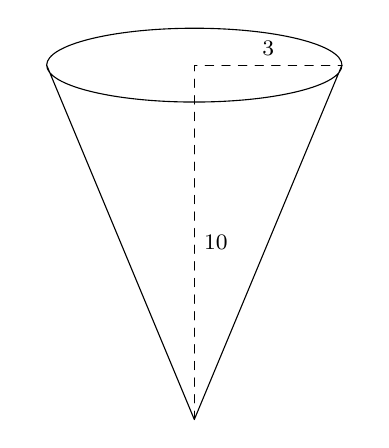
\begin{tikzpicture}[scale=.75, font=\footnotesize, line join=round, line cap=round, >=stealth]
				\def\x{2.5} % Bán kính trụ lớn
				\pgfmathsetmacro{\y}{\x/4} % Bán kính trục bé
				\def\h{6} % Chiều cao
				\coordinate[label=below:] (O) at (0,0);
				\coordinate[label=right:] (C) at (\x,0);
				\coordinate[label=above:] (A) at (0,-\h);
				\coordinate[label=left:] (B) at (-\x,0);
				%\coordinate[label=below left:$D$] (D) at ($(O)+(240:{\x} and {\y})$);
				%\coordinate[label=below:$\text{Hình 3}$] (F) at ($(O)+(-90:1)$);	
				\draw (C) arc (0:-360:{\x} and {\y})--(A)--(B)
				;
				\draw[dashed] (A)--(O)node[midway, right]{$10$}--(C)node[midway, above]{$3$};
				%\foreach \diem in {A,C,O,B,D}	\fill (\diem)circle(1.5pt);
				%\draw pic[draw,blue,angle radius=3mm] {right angle = C--O--A}; 
		\end{tikzpicture}}
	}
\end{bt}

\begin{bt}%[Dự án EX-9-Đề Cương Toán 9]%[Phạm Hoài]%[9H4V2-4]
	Bác Hà thuê xe cải tiến (Hình a) chuyển một đống cát có dạng hình nón với chu vi đáy $9{,}42$ m và chiều cao là $1{,}2$ m (Hình b) để xây tường nhà. Biết thùng chứa của xe có dạng hình hộp chữ nhật với kích thước dài $1{,}57$ m, rộng $0{,}8$ m và cao $0{,}4$ m. Trong mỗi chuyến xe, bác Hà chở lượng cát ít hơn thể tích thực của xe là $5 \%$. Hỏi bác Hà cần phải chuẩn bị ít nhất bao nhiêu tiền để chuyển hết đống cát trên, biết rằng giá vận chuyển của một chuyến xe là $90\,000$ đồng?
	\begin{center}
		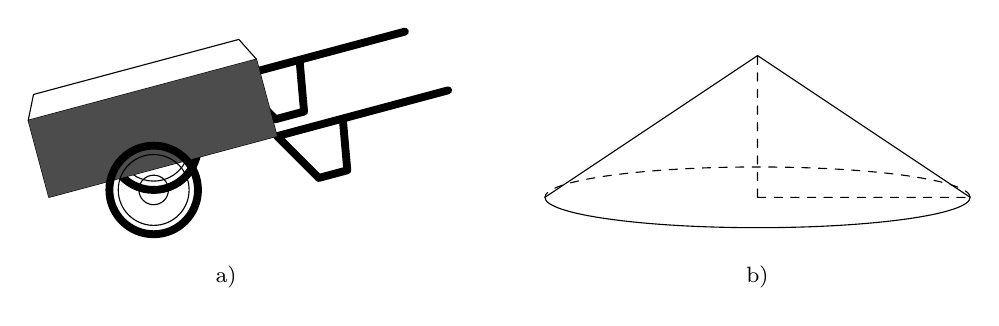
\begin{tikzpicture}[scale=.75,font=\footnotesize, line join=round, line cap=round, >=stealth]
			\def\r{3}
			\def\h{2}
			%Vẽ hình nón
			\begin{scope}[scale=1.2]
				\draw[dashed] (0:\r) arc(0:180:{\r} and {\r/7})
				(0:0)--++(0:\r)
				(0,0)--++(90:\h)
				;
				\draw (0:\r) arc(360:180:{\r} and {\r/7})
				(-\r,0)--(0,\h)--(\r,0);
			\end{scope}
			
			\begin{scope}[shift={(-12,0)}]
				\begin{scope}[scale=.5,shift={(3.55,1.75)}]
					\draw (0,0) circle (1.2) circle (0.5);
					\draw[fill] (0,0) circle (.1) ;	
					\draw[line width=1mm] (0,0) circle(1.5);
				\end{scope}
				
				
				\begin{scope}[rotate=15]
					\draw[line width=1mm] (4,0)--(7,0) (4,0)--++(-60:1)--++(0:.5)--++(80:.85) ;
					\draw[line width=1mm,shift={(-.45,1.15)}] (4,0)--(7,0) (4,0)--++(-60:1)--++(0:.5)--++(80:.85) ;
				\end{scope}
				
				\begin{scope}[rotate=15]
					\draw (0,0)--(4,0)--(4,1.35)--(0,1.35)--(0,0);
					\fill[black!70] (0,0)--(4,0)--(4,1.35)--(0,1.35)--(0,0);
					\draw (4,1.35)--(3.8,1.75) --(0.2,1.75)--(0,1.35);
				\end{scope}
				
				\begin{scope}[scale=.5,shift={(3.55,.25)}]
					\draw (0,0) circle (1.2) circle (0.5);
					\draw[fill] (0,0) circle (.1) ;	
					\draw[line width=1mm] (0,0) circle(1.5);
				\end{scope}
			\end{scope}
			\fill (0,-1) node[below]{b)};
			\fill (-9,-1) node[below]{a)};
		\end{tikzpicture}
	\end{center}
	\loigiai{
		Ta có chu vi đáy của đống cát là $C=2\pi r=9{,}42$ suy ra $r=\dfrac{9{,}42}{2\pi} = \dfrac{471}{100\pi}$ (m).\\
		Thể tích đống cát là $V=\dfrac{1}{3}\pi r^2 h =\dfrac{1}{3}\pi \left(\dfrac{471}{100\pi}\right)^2\cdot 1{,}2\approx 2{,}82$ (m$^2$).\\
		Thể tích thùng chứa của xe bằng $1{,}57\cdot 0{,}8\cdot 0{,}4=0{,}5024$ (m$^2$).\\
		Lượng cát của một lần chuyển bằng $95\%\cdot 0{,}5024 = 0{,}47728$ (m$^2$).\\
		Số lần vận chuyển để chuyển hết đống cát là $\dfrac{2{,}82}{0{,}47728}\approx 5{,}9$ (lần).\\
		Vậy cần ít nhất $6$ lần để chuyển hết đống cát.\\
		Vậy bác Hà cần chuẩn bị ít nhất $90\,000\cdot 6 = 540\,000$ đồng để chuyển hết đống cát.
	}
\end{bt}

\begin{bt}%[Dự án EX-9-Đề Cương Toán 9]%[Phạm Hoài]%[9H4H4-1]
	\immini{Bác Khôi làm một dụng cụ bằng tôn gồm một phần có dạng hình trụ và một phần có dạng hình nón với các kích thước như (Hình bên). Tính thể tích của dụng cụ này (\textit{coi mép hàn không đáng kể và làm tròn kết quả đến hàng đơn vị của cm$^3$}).}{
		\begin{tikzpicture}[scale=0.7, font=\footnotesize,>=stealth, rotate=90]
			%Gán số liệu.
			\def\a{2};\def\b{0.7};\def\h{4};
			%Gán tọa độ.
			\coordinate (O) at (0,0);
			\coordinate (O') at ($(O)+(90:\h)$);
			\coordinate (A) at ($(O)-(0:\a)$);
			\coordinate (B) at ($(O)+(0:\a)$);
			\coordinate (A') at ($(A)+(90:\h)$);
			\coordinate (B') at ($(B)+(90:\h)$);
			\coordinate (O1) at ($(O')!1.8!(O)$);
			\coordinate (B1) at ($(B)+1*(O1)-1*(O)$);
			%Vẽ khối trụ.
			\draw (B) arc (0:-180:\a cm and \b cm)(B') arc (0:-180:\a cm and \b cm) (A)--(A') (B)--(B') (A')--(B') (B') arc (0:180:\a cm and \b cm);
			\draw[dashed] (B) arc (0:180:\a cm and \b cm) (O1)--(B1);
			\draw(A)--(O1)--(B);
			\draw[|<->|](B')--(B)node[sloped, midway, sloped, above,rotate=90]{$30$ cm};
			\draw[|<->|](B)--(B1)node[sloped, midway, sloped, above,rotate=-90]{$20$ cm};
			\draw[|<->|](A')--(B')node[sloped, midway, sloped, above,rotate=90]{$20$ cm};
			%Gán nhãn.
			%\foreach \x/\y in {O/45, O'/45, A/180, B/0, A'/180, B'/0, O1/0}{\fill (\x) circle(1pt) ($(\x)+(\y:0.3cm)$) node{$\x$};}
		\end{tikzpicture}
	}
	\loigiai{
		Thể tích của hình trụ là \[V_1=\pi\cdot 10^2\cdot 30=3\,000\pi \text{ (cm$^3$).}\]
		Thể tích của hình nón là 
		\[V_2=\dfrac{1}{3}\pi\cdot 10^2\cdot 20=\dfrac{2\,000\pi}{3} \text{ (cm$^3$).}\]
		Thể tích của dụng cụ này là 
		\[V=V_1+V_2=3000 \pi+\dfrac{2\,000}{3} \pi=\dfrac{11\,000}{3} \pi\approx 11\,519 \text{ (cm$^3$).}\]
	}
\end{bt}


\begin{bt}%[Dự án EX-9-Đề Cương Toán 9]%[Phạm Hoài]%[9H4V2-4]
	\immini{Một cái mũ chú hề có kích thước như hình bên. Hãy tính tổng diện tích giấy làm nên chiếc mũ (\textit{không tính phần hao hụt, kết quả làm tròn đến hàng đơn vị}).}
	{\begin{tikzpicture}[scale=0.5,>=stealth]
			%		\tkzDefPoints{0/0/O'} 
			\def\a{3} % bán trục lớn = bán kính trụ
			\def\b{1} % bán trục nhỏ
			\def\c{6} % bán trục lớn = bán kính trụ
			\def\d{2}
			\def\h{4} % chiều cao trụ
			\draw[dashed,line width=1pt] (\a,0) arc [x radius=\a, y radius=\b, start angle=0, end angle=150];
			\draw [line width=1pt](\a,0) arc [x radius=\a, y radius=\b, start angle=0, end angle=-205];
			\draw[dashed,line width=1pt] (\c,0) arc [x radius=\c, y radius=\d, start angle=0, end angle=110];
			\draw [line width=1pt](\c,0) arc [x radius=\c, y radius=\d, start angle=0, end angle=-251];
			\draw [line width=1pt](\c,0) arc [x radius=\c, y radius=\d, start angle=0, end angle=71];
			\draw[<->,line width=1pt]($(O)+(180:\a)$)--($(O)+(180:\a)+(-3,0)$);
			\draw[<->,line width=1pt] (-6,-2.2)--(6,-2.2);
			\draw(-4.5,0.4) node {$10\text{\;cm}$}(0,-2.6) node {$35\text{\;cm}$}(2.75,2.75) node {$30\text{\;cm}$};
			\draw[line width=1pt] (-\a,0)--(0,1.5*\h)--(\a,0);
	\end{tikzpicture}}
	\loigiai{
		Bán kính hình tròn là $r=\dfrac{d}{2}=\dfrac{35}{2}$ (cm).\\
		Bán kính hình nón bằng $r_{\text{nón}}=\dfrac{35}{2}-10=\dfrac{15}{2}$ (cm).\\
		Diện tích hình vành khăn bằng $S_{\text{vành khăn}}=\pi\left[\left(\dfrac{35}{2}\right)^2-\left(\dfrac{15}{2}\right)^2\right]=250\pi$ (cm$^2$).\\
		Diện tích xung quanh của hình nón là $S_{\text{xq}}=\pi r_{\text{nón}}l =\pi\cdot \dfrac{15}{2}\cdot 30 = 225\pi$ (cm$^2$).\\
		Tổng diện tích giấy làm nên chiếc mũ bằng $S=S_{\text{vành khăn}}+S_{\text{xq}}=250\pi+225\pi\approx1\,492$ (cm$^2$).
	}
\end{bt}

\begin{bt}%[Dự án EX-9-Đề Cương Toán 9]%[Phạm Hoài]%[9H4V2-3]
	Trong các phát biểu sau, phát biểu nào \textbf{sai}?
	\begin{enumerate}
		\item Nếu bán kính đáy của một hình nón tăng lên hai lần và giữ nguyên chiều cao thì thể tích của hình nón đó sẽ tăng lên hai lần.
		\item Nếu chiều cao của một hình nón tăng lên hai lần và giữ nguyên bán kính đáy thì thể tích của hình nón đó sẽ tăng lên hai lần.
		\item Nếu bán kính đáy và chiều cao của một hình nón cùng tăng lên hai lần thì thể tích của hình nón đó sẽ tăng lên bốn lần.
	\end{enumerate}
	\loigiai{
		\begin{enumerate}
			\item Gọi $r'$, $V'$ lần lượt là bán kính đáy và thể tích lúc sau của hình nón.\\
			Ta có $\dfrac{V'}{V}=\dfrac{\dfrac{1}{3}\pi r'^2 h}{\dfrac{1}{3} \pi r^2 h}=\left(\dfrac{r'}{r}\right)^2=2^2=4$. \\
			Vậy $V'=4V$ nên phát biểu này sai.
			\item Gọi $h'$, $V'$ lần lượt là chiều cao và thể tích lúc sau của hình nón.\\
			Ta có $\dfrac{V'}{V}=\dfrac{\dfrac{1}{3}\pi r^2 h'}{\dfrac{1}{3} \pi r^2 h}=\dfrac{h'}{h}=2$.\\ Vậy $V'=2V$ nên phát biểu này đúng.
			\item Gọi $r'$, $h'$, $V'$ lần lượt là bán kính đáy, chiều cao và thể tích lúc sau của hình nón.\\
			Ta có $\dfrac{V'}{V}=\dfrac{\dfrac{1}{3}\pi r'^2 h'}{\dfrac{1}{3} \pi r^2 h}=\left(\dfrac{r'}{r}\right)^2\dfrac{h'}{h}=2^2\cdot 2=8$.\\
			Vậy $V'=8V$ nên phát biểu này sai.
		\end{enumerate}
	}
\end{bt}

\begin{bt}%[Dự án EX-9-Đề Cương Toán 9]%[Phạm Hoài]%[9H4C2-3]
	\immini{Hình bên minh hoạ hình nón đỉnh $B$ với đường cao $BH$ và hình nón đỉnh $C$ với đường cao $CH$ có chung đường tròn đáy tâm $H$.
	\begin{enumerate}
		\item Chứng minh rằng: tỉ số thể tích của hình nón đỉnh $B$ và thể tích của hình nón đỉnh $C$ bằng tỉ số đường cao $BH$ và đường cao $CH$.
		\item Phát biểu sau đúng hay sai: \lq\lq Tỉ số thể tích hai hình nón có cùng bán kính đường tròn đáy bằng tỉ số hai đường cao tương ứng của hai hình nón đó\rq\rq? Vì sao?
	\end{enumerate}
	}{
	\begin{tikzpicture}[scale=.75, font=\footnotesize, line join=round, line cap=round, >=stealth]
			\def\x{3} % Bán kính trụ lớn
			\pgfmathsetmacro{\y}{\x/4} % Bán kính trục bé
			\def\h{3} % Chiều cao
			\coordinate[label=right:$H$] (H) at (0,0);
			\coordinate[label=right:$C$] (C) at (0,-4);
			\coordinate[label=above:$B$] (B) at (0,\h);
			\coordinate[label=left:] (A) at (\x,0);
			\coordinate[label=below left:] (D) at (-\x,0);
			\coordinate[label=below:$ $] (F) at ($(C)+(-90:1)$);	
			\draw (A) arc (0:-180:{\x} and {\y})--(B)--(A)--(C)--(D)
			;
			\draw[dashed] (B)--(C);
			\draw[dashed] (A) arc (0:180:{\x} and {\y});
			\foreach \diem in {B,H,C}	\fill (\diem)circle(1.5pt);
			%\draw pic[draw,blue,angle radius=3mm] {right angle = C--O--A}; 
	\end{tikzpicture}}
	\loigiai{
		\begin{enumerate}
			\item Gọi $V_1$, $V_2$ lần lượt là thể tích của hình nón đỉnh $B$ và hình nón đỉnh $C$. \\
			Ta có $V_1=\dfrac{1}{3}\pi r^2 BH$ và $V_2=\dfrac{1}{3}\pi r^2 CH$.\\
			 Suy ra $\dfrac{V_1}{V_2}=\dfrac{\dfrac{1}{3}\pi r^2 BH}{\dfrac{1}{3}\pi r^2 CH}=\dfrac{BH}{CH}$.
			\item Gọi $V_1$, $h_1$; $r_1$, $V_2$, $h_2$, $r_2$ lần lượt là thể tích, chiều cao và bán kính đáy của hình nón đỉnh $B$ và hình nón đỉnh $C$.\\
			Ta có $V_1=\dfrac{1}{3}\pi r_1^2 h_1$ và $V_2=\dfrac{1}{3}\pi r_2^2 h_2$. \\
			Suy ra $\dfrac{V_1}{V_2}=\dfrac{\dfrac{1}{3}\pi r_1^2 h_1}{\dfrac{1}{3}\pi r_2^2 h_2}=\dfrac{h_1}{h_2}$ (do $r_1=r_2$). \\
			Vậy phát biểu trên là phát biểu đúng.
		\end{enumerate}
	}
\end{bt}

